\documentclass[pdftex]{beamer}
\usepackage[british]{babel}
\usepackage{graphicx}
\usepackage{url}
\usepackage[normalem]{ulem}
\usepackage{tikz}

\mode<presentation>
\usetheme{Warsaw}
\useoutertheme{infolines}

\setbeamertemplate{navigation symbols}{}
% \usebeamertemplate*{logo}
% \logo{
\includegraphics[height=0.85cm]{../images/cmetlogo.png}}

\title[Exploring UK Crime Networks]{{\huge{Exploring UK Crime Networks}}}
\author[FOSINT-SI 2014]{Giles Oatley and Tom Crick\\\url{tcrick@cardiffmet.ac.uk}}
\institute[@DrTomCrick]{Department of Computing \& Information
  Systems\\Cardiff Metropolitan University, UK\\\url{http://drtomcrick.com}}
\date{18 August 2014}

% logo  on title page only
\titlegraphic{
\includegraphics[width=4cm]{../images/cmetlogo.png}
}

\begin{document}

% titlepage
\begin{frame}
\titlepage
\end{frame}

% TOC
\section*{Talk Outline} 
\begin{frame} 
\tableofcontents 
\end{frame} 

\section{Introduction and Motivation}

\begin{frame}
\frametitle{Abstract}
{\emph{This paper describes our experiences with three different crime
networks in the UK: burglary, ‘gun’ gangs and retail theft. We present
an introduction into each of these problems, and highlight some of the
issues related to over- simplification of the network analysis.\newline

We also review the term ‘third-generation’ analysis, and provide some
insights into achieving this, but also conclude that it can be an
extremely expensive (computational/analytical) undertaking.}}
\end{frame}

\section{Crime Analysis Techniques}

\begin{frame}
\frametitle{Crime Analysis Techniques}
\begin{itemize}
\item {\textbf{First Generation}}
\begin{itemize}
\item Anacpapa charts
\item Maps with coloured pins\newline
\end{itemize}
\pause
\item {\textbf{Second Generation}}
\begin{itemize}
\item Pajek
\item IBM i2 COPLINK2, IBM i2 Analyst’s Notebook3, ORA
\item Detica NetReveal\newline
\end{itemize}
\pause
\item {\textbf{Third Generation?}}
\end{itemize}
\end{frame}

\begin{frame}
\frametitle{Crime Analysis Techniques}
``{\emph{Social network analysis of the sort we could call ‘third-generation’
would focus much more intensely on the content of the contacts, on the
social context, and on the interpretation of such information.}}''
(Klerks, 2001)\newline\newline

...understanding in a qualitative way the {\textbf{behaviour, motivations and
choices}} of the individuals concerned and contributing to a better
understanding of vital {\textbf{social processes, power and affinity structures}}.
\end{frame}

\section{UK Crime Networks}

\begin{frame}
\frametitle{UK Crime Networks}
{\Large{
\begin{enumerate}
\item Burglary\newline
\item Gun Gangs\newline
\item Retail Theft\newline
\end{enumerate}}}
\end{frame}

\subsection{Burglary}

\begin{frame}
\frametitle{Burglary}
\begin{itemize}
\item In conjunction with {\textbf{West Midlands Police, UK}}
\item Large network of linked offenders ({\emph{n}}=17000)
\item The picture painted by the initial social network plot is
somewhat misleading...
\item While betweenness metric useful, need to consider spatial and other features (temporal/frequency) to
  start to understand the meaning of the links between offenders
\end{itemize}
\end{frame}

% { % all template changes are local to this group.
%     \setbeamertemplate{navigation symbols}{}
%     \begin{frame}[plain]
%         \begin{tikzpicture}[remember picture,overlay]
%             \node[at=(current page.center)] {
%                 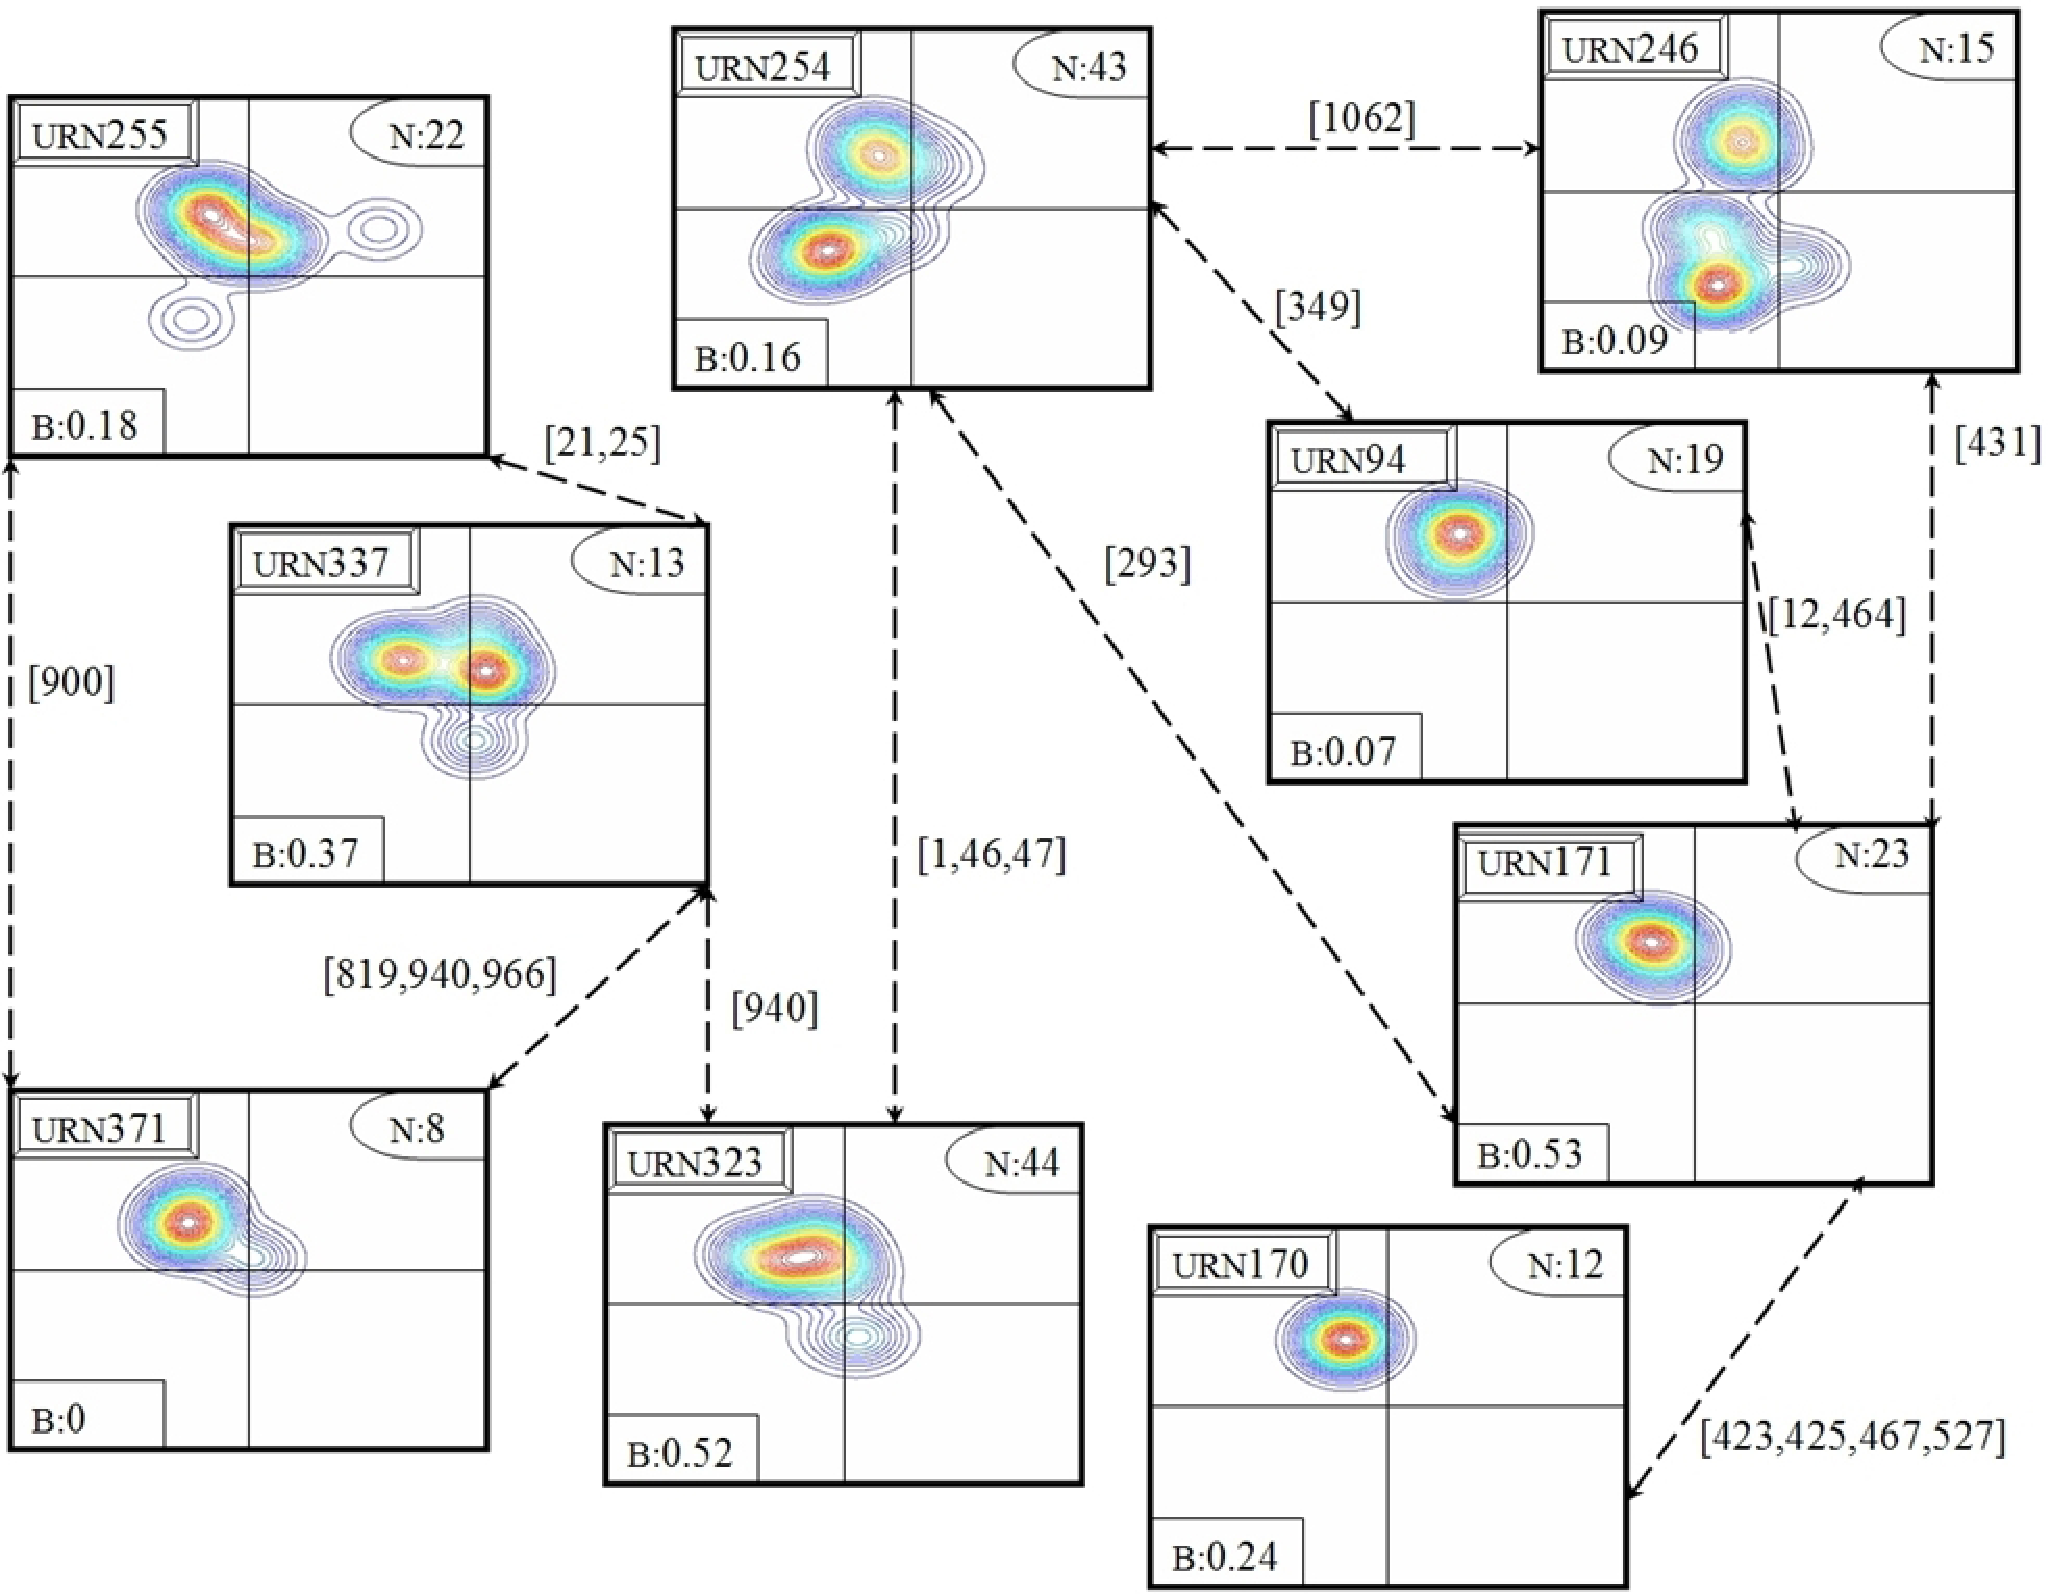
\includegraphics[width=0.9\paperwidth]{../images/burglary.pdf}
%             };
%         \end{tikzpicture}
%      \end{frame}
% }

\begin{frame}
%\frametitle{Geographical Networks of Burglars}
\begin{center}
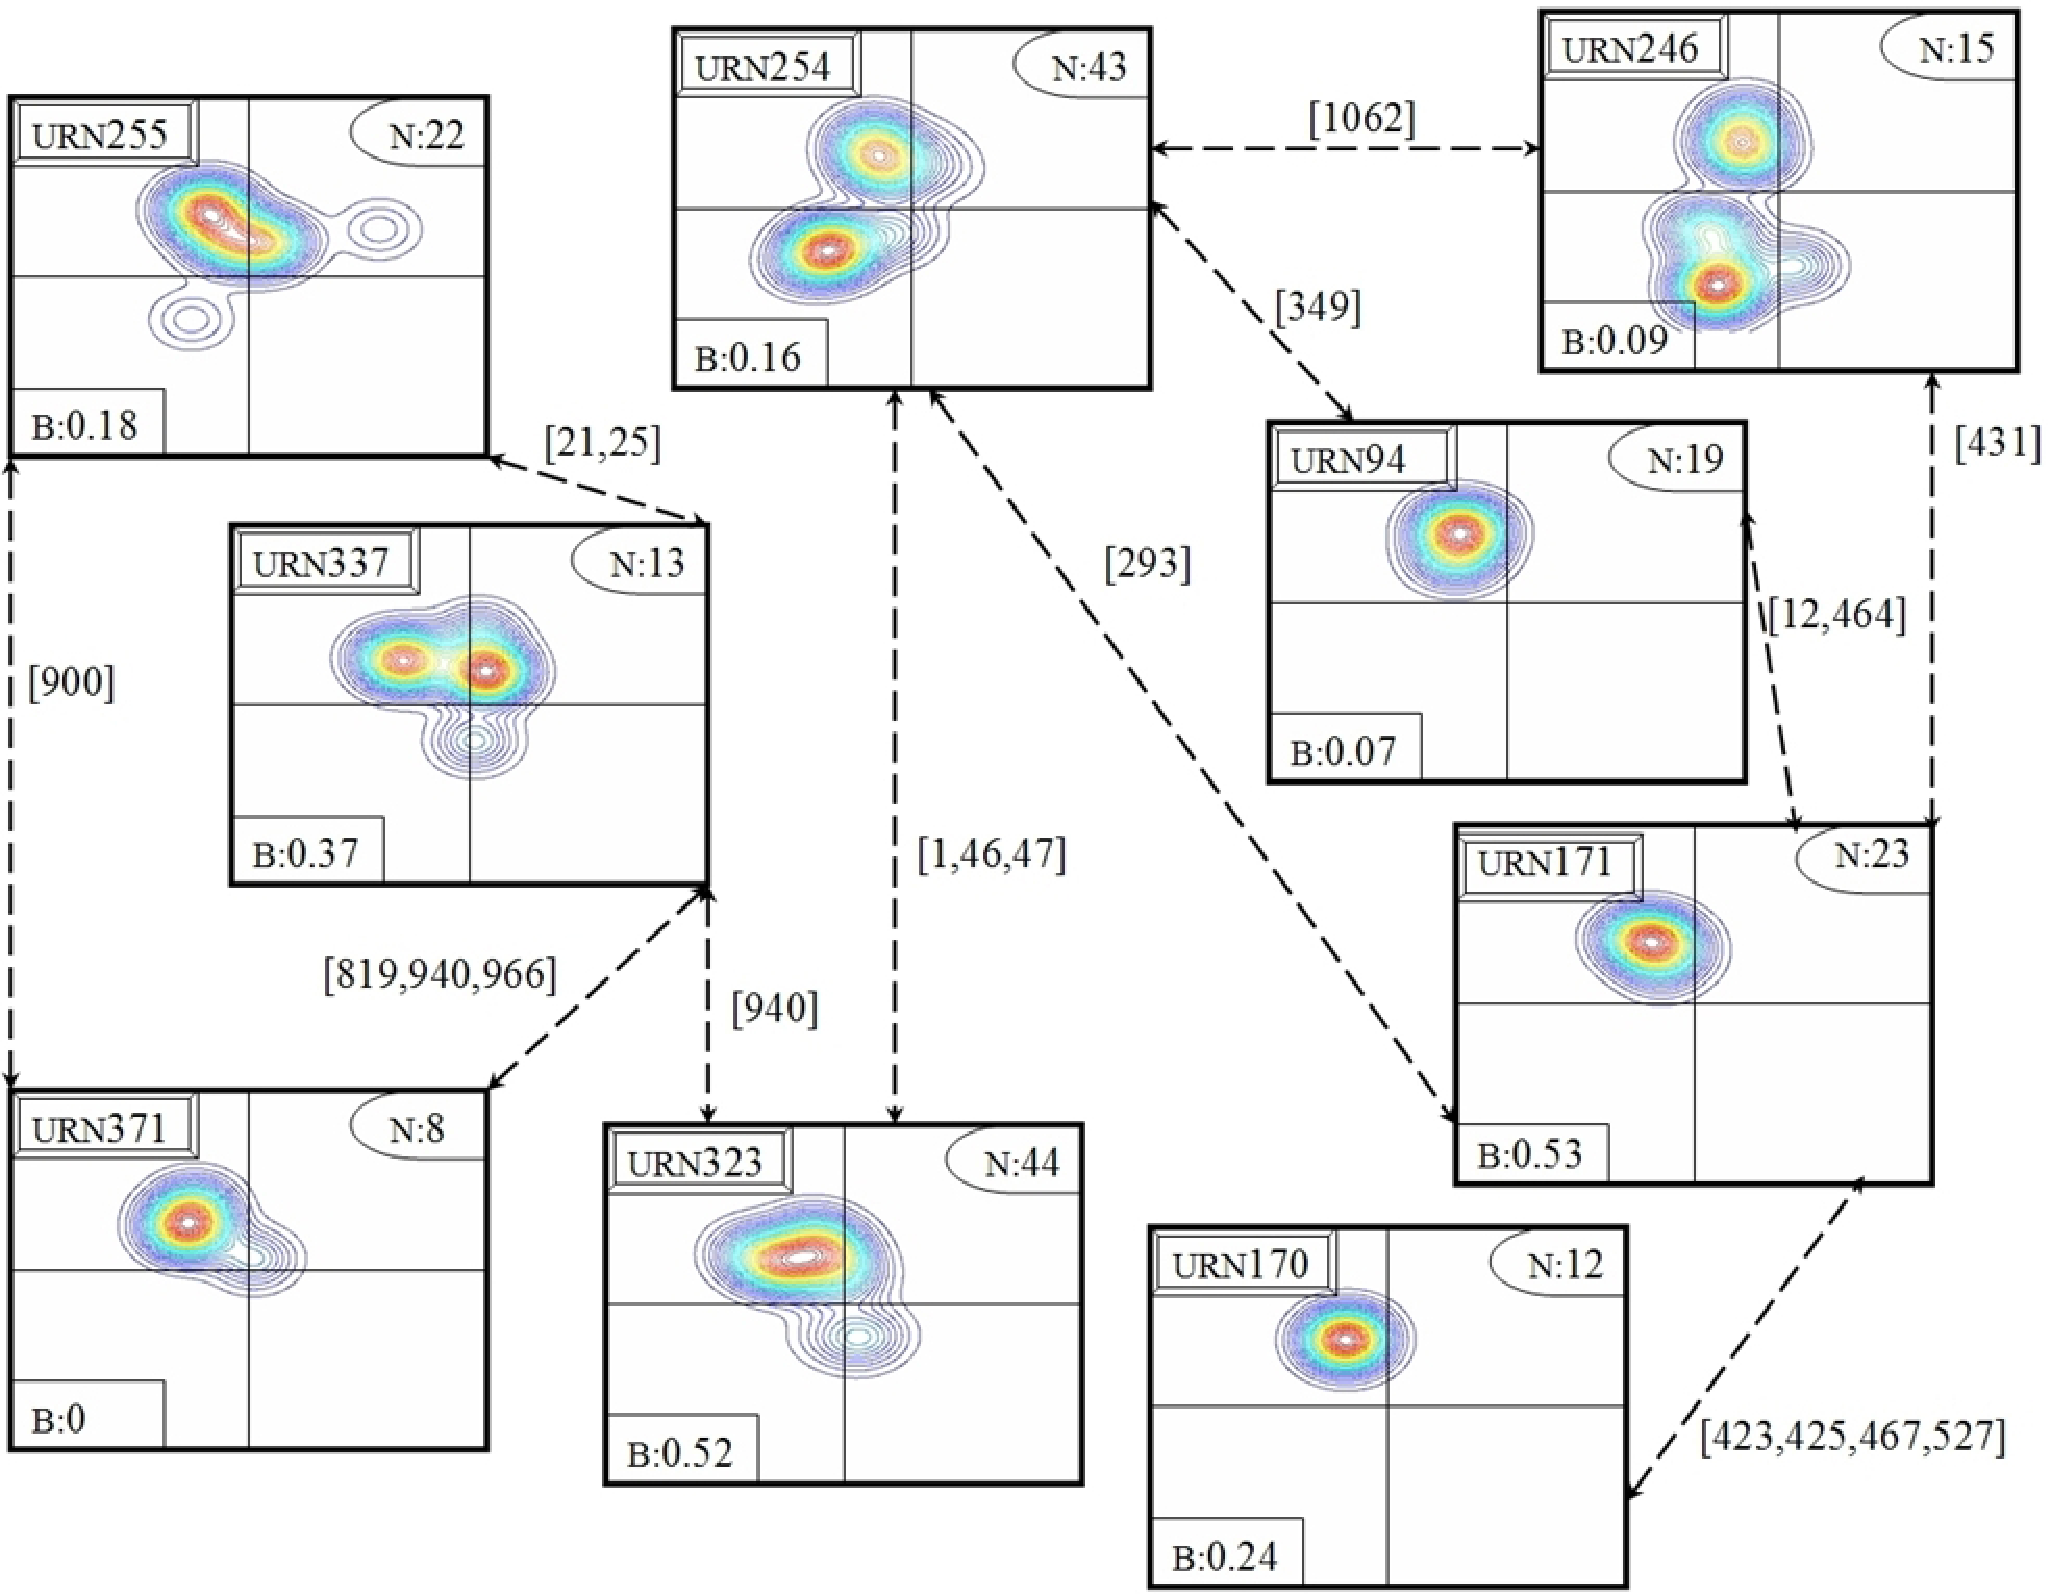
\includegraphics[width=0.7\paperwidth]{../images/burglary.pdf}
\end{center}
\scriptsize{{\textbf{Geographical networks of burglars.}} Each of the 2x2 squares represents an offender, with
  Unique Reference Number (URN), number of crimes (N) and betweeness
  value (B). The links between offenders are labelled with dates, as days from the start of the project.}
\end{frame}

\subsection{Gun Gangs}

{ % all template changes are local to this group.
    \setbeamertemplate{navigation symbols}{}
    \begin{frame}[plain]
        \begin{tikzpicture}[remember picture,overlay]
            \node[at=(current page.center)] {
                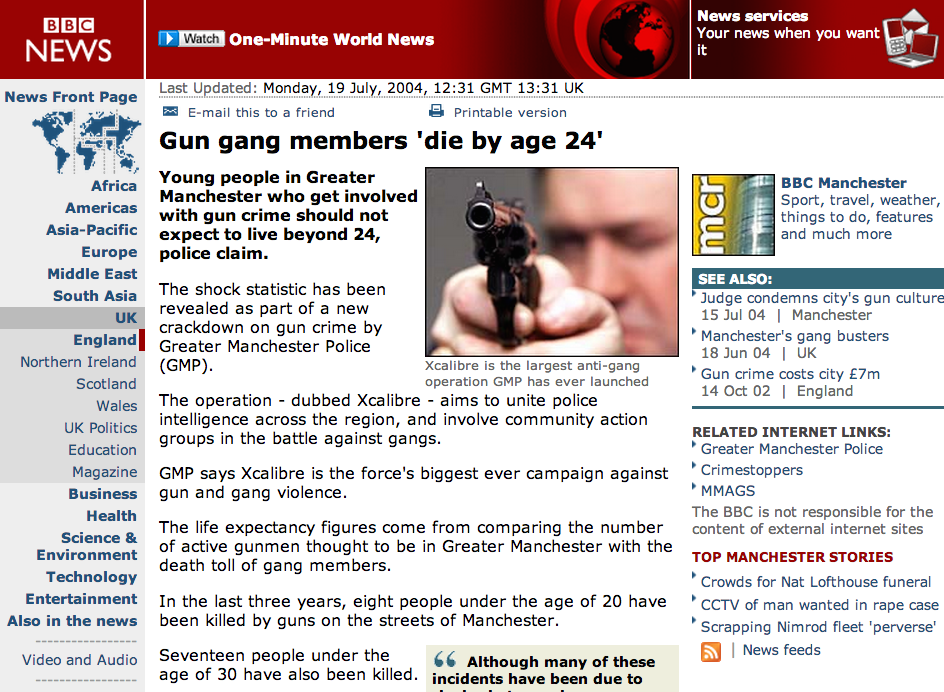
\includegraphics[width=\paperwidth]{../images/bbcnewsmanc2004.png}
            };
        \end{tikzpicture}
     \end{frame}
}

\begin{frame}
\frametitle{Gun Gangs}
\begin{itemize}
\item In conjunction with {\textbf{Greater Manchester Police, UK}}
\item Area with a significant gun crime problem, related to gang activity
\item Dynamics of four gangs and their associates
\item Value of SNA for gang research:
\begin{itemize}
\item Identifying structural holes
\item Betweenness
\item Social capital
\end{itemize}
\item Value of third generation analysis
\end{itemize}
\end{frame}

% { % all template changes are local to this group.
%     \setbeamertemplate{navigation symbols}{}
%     \begin{frame}[plain]
%         \begin{tikzpicture}[remember picture,overlay]
%             \node[at=(current page.center)] {
%                 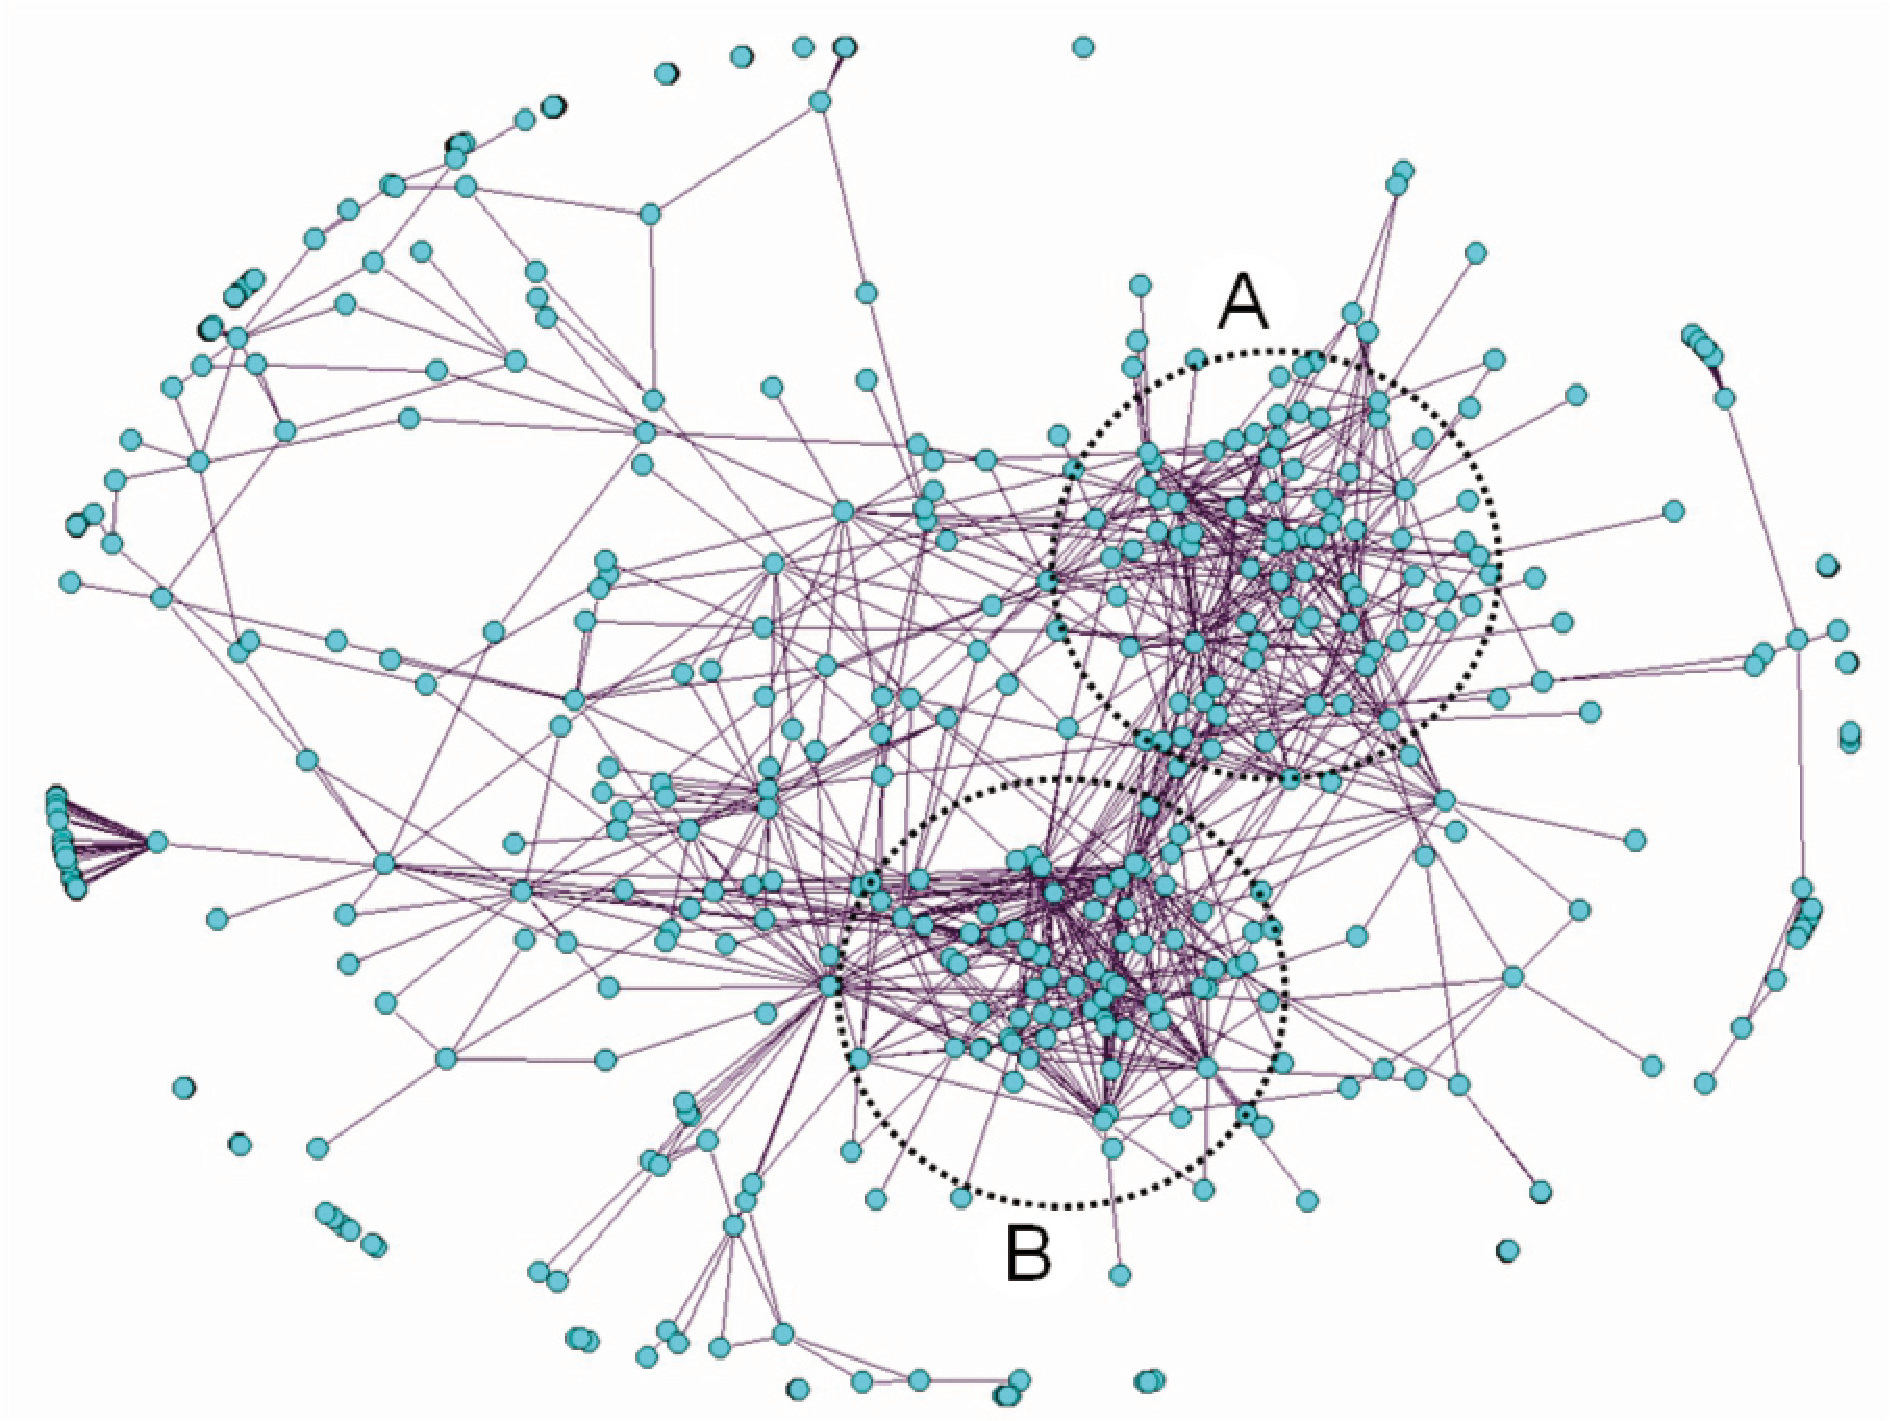
\includegraphics[width=0.9\paperwidth]{../images/2000ganglabels.pdf}
%             };
%         \end{tikzpicture}
%      \end{frame}
% }

\begin{frame}
\begin{center}
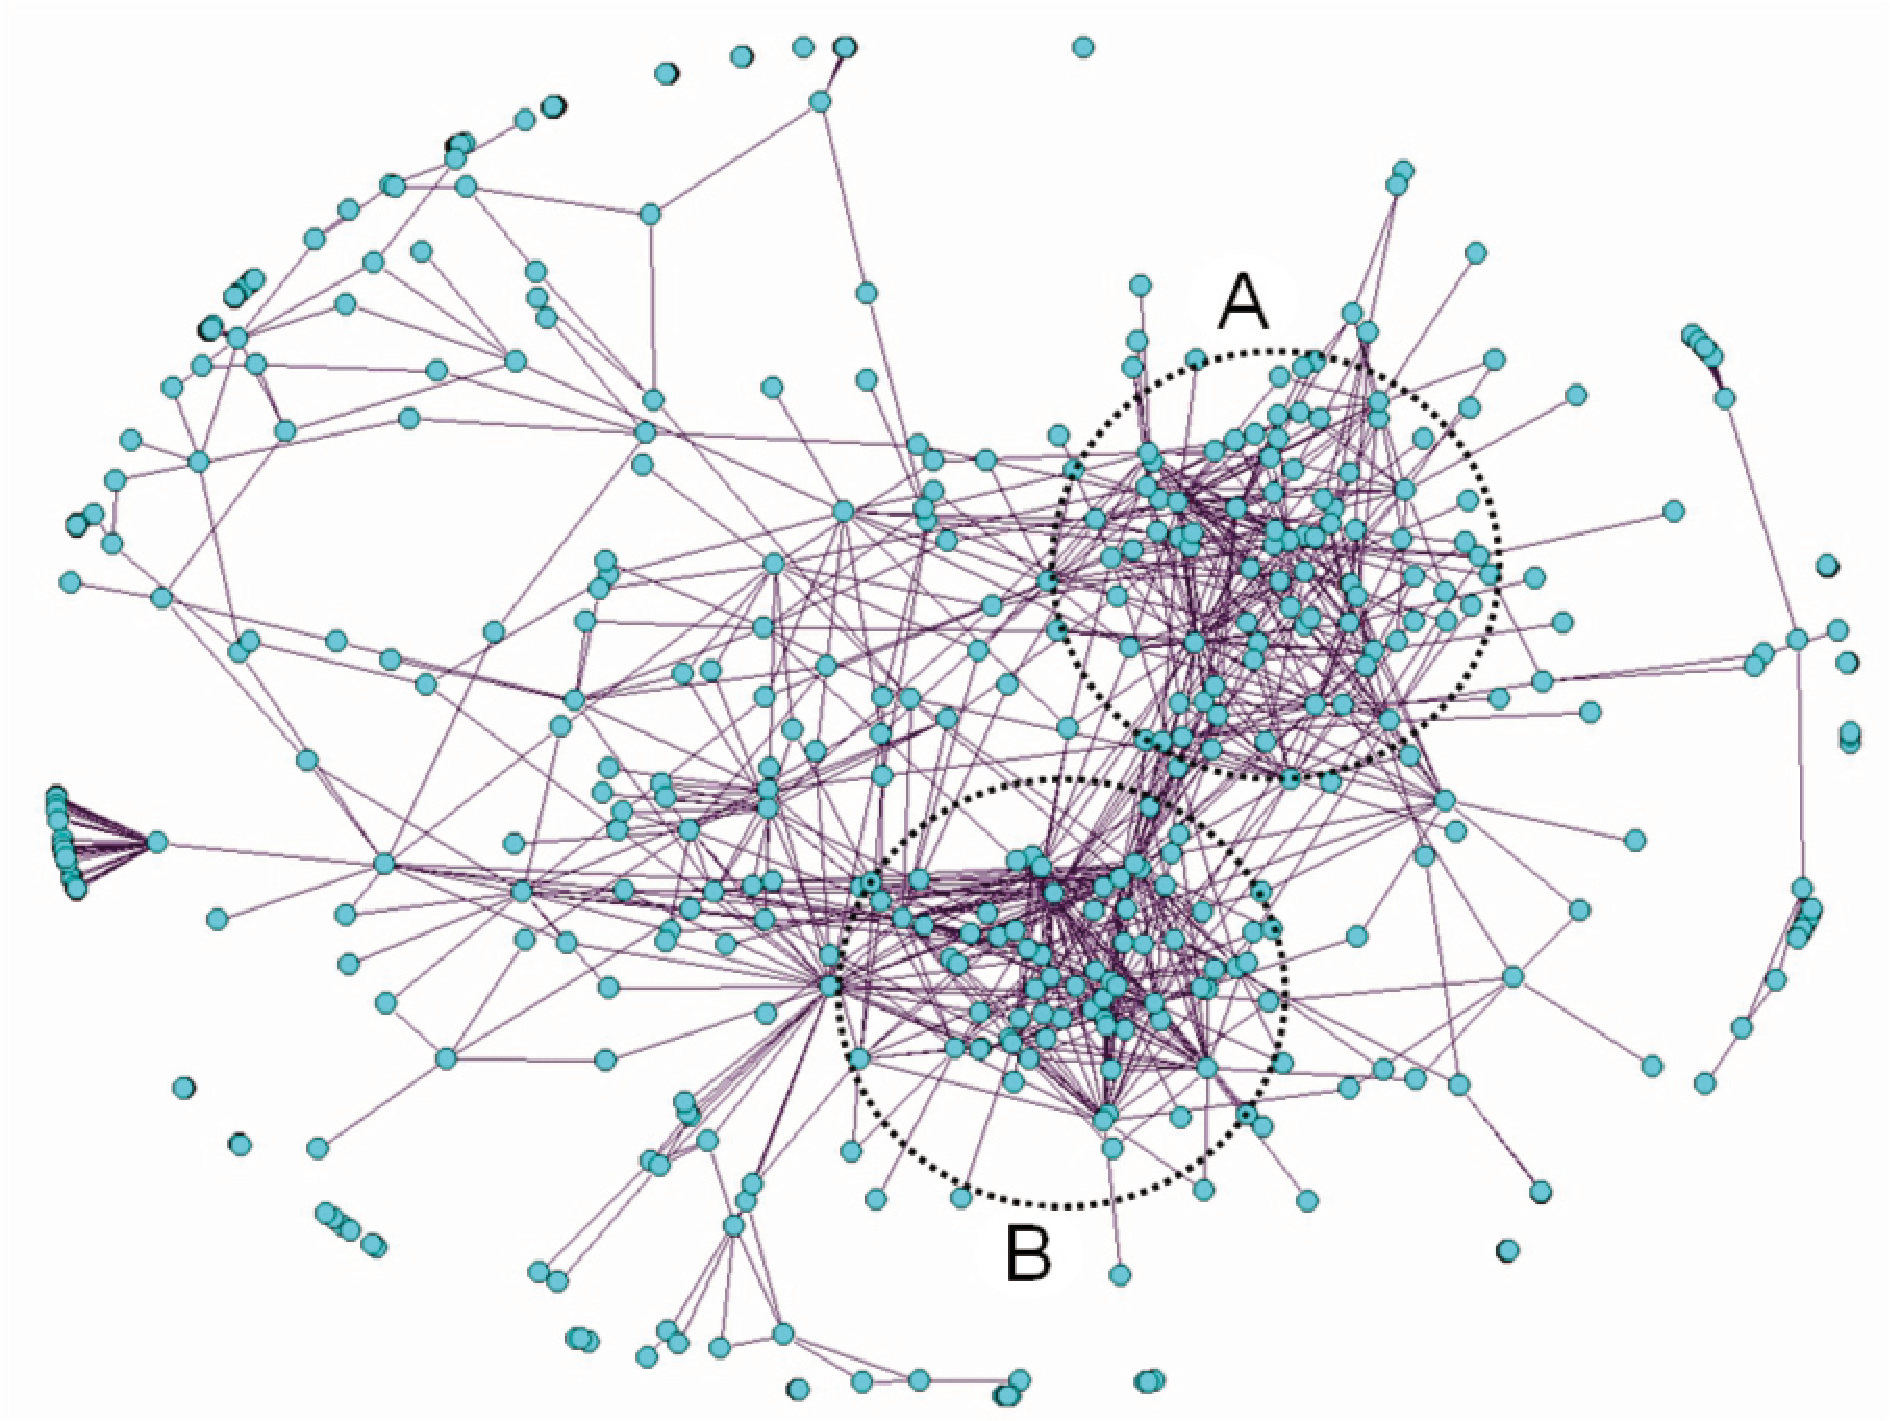
\includegraphics[width=0.8\paperwidth]{../images/2000ganglabels.pdf}
\end{center}
\scriptsize{{\textbf{Links between two rival gangs A and B.}} In 2000,
  Gangs A and B were rivals. These later divided in 2001 into Gang C
  (from A) and into Gang D (from B) in 2004.}
\end{frame}

{ % all template changes are local to this group.
    \setbeamertemplate{navigation symbols}{}
    \begin{frame}[plain]
        \begin{tikzpicture}[remember picture,overlay]
            \node[at=(current page.center)] {
                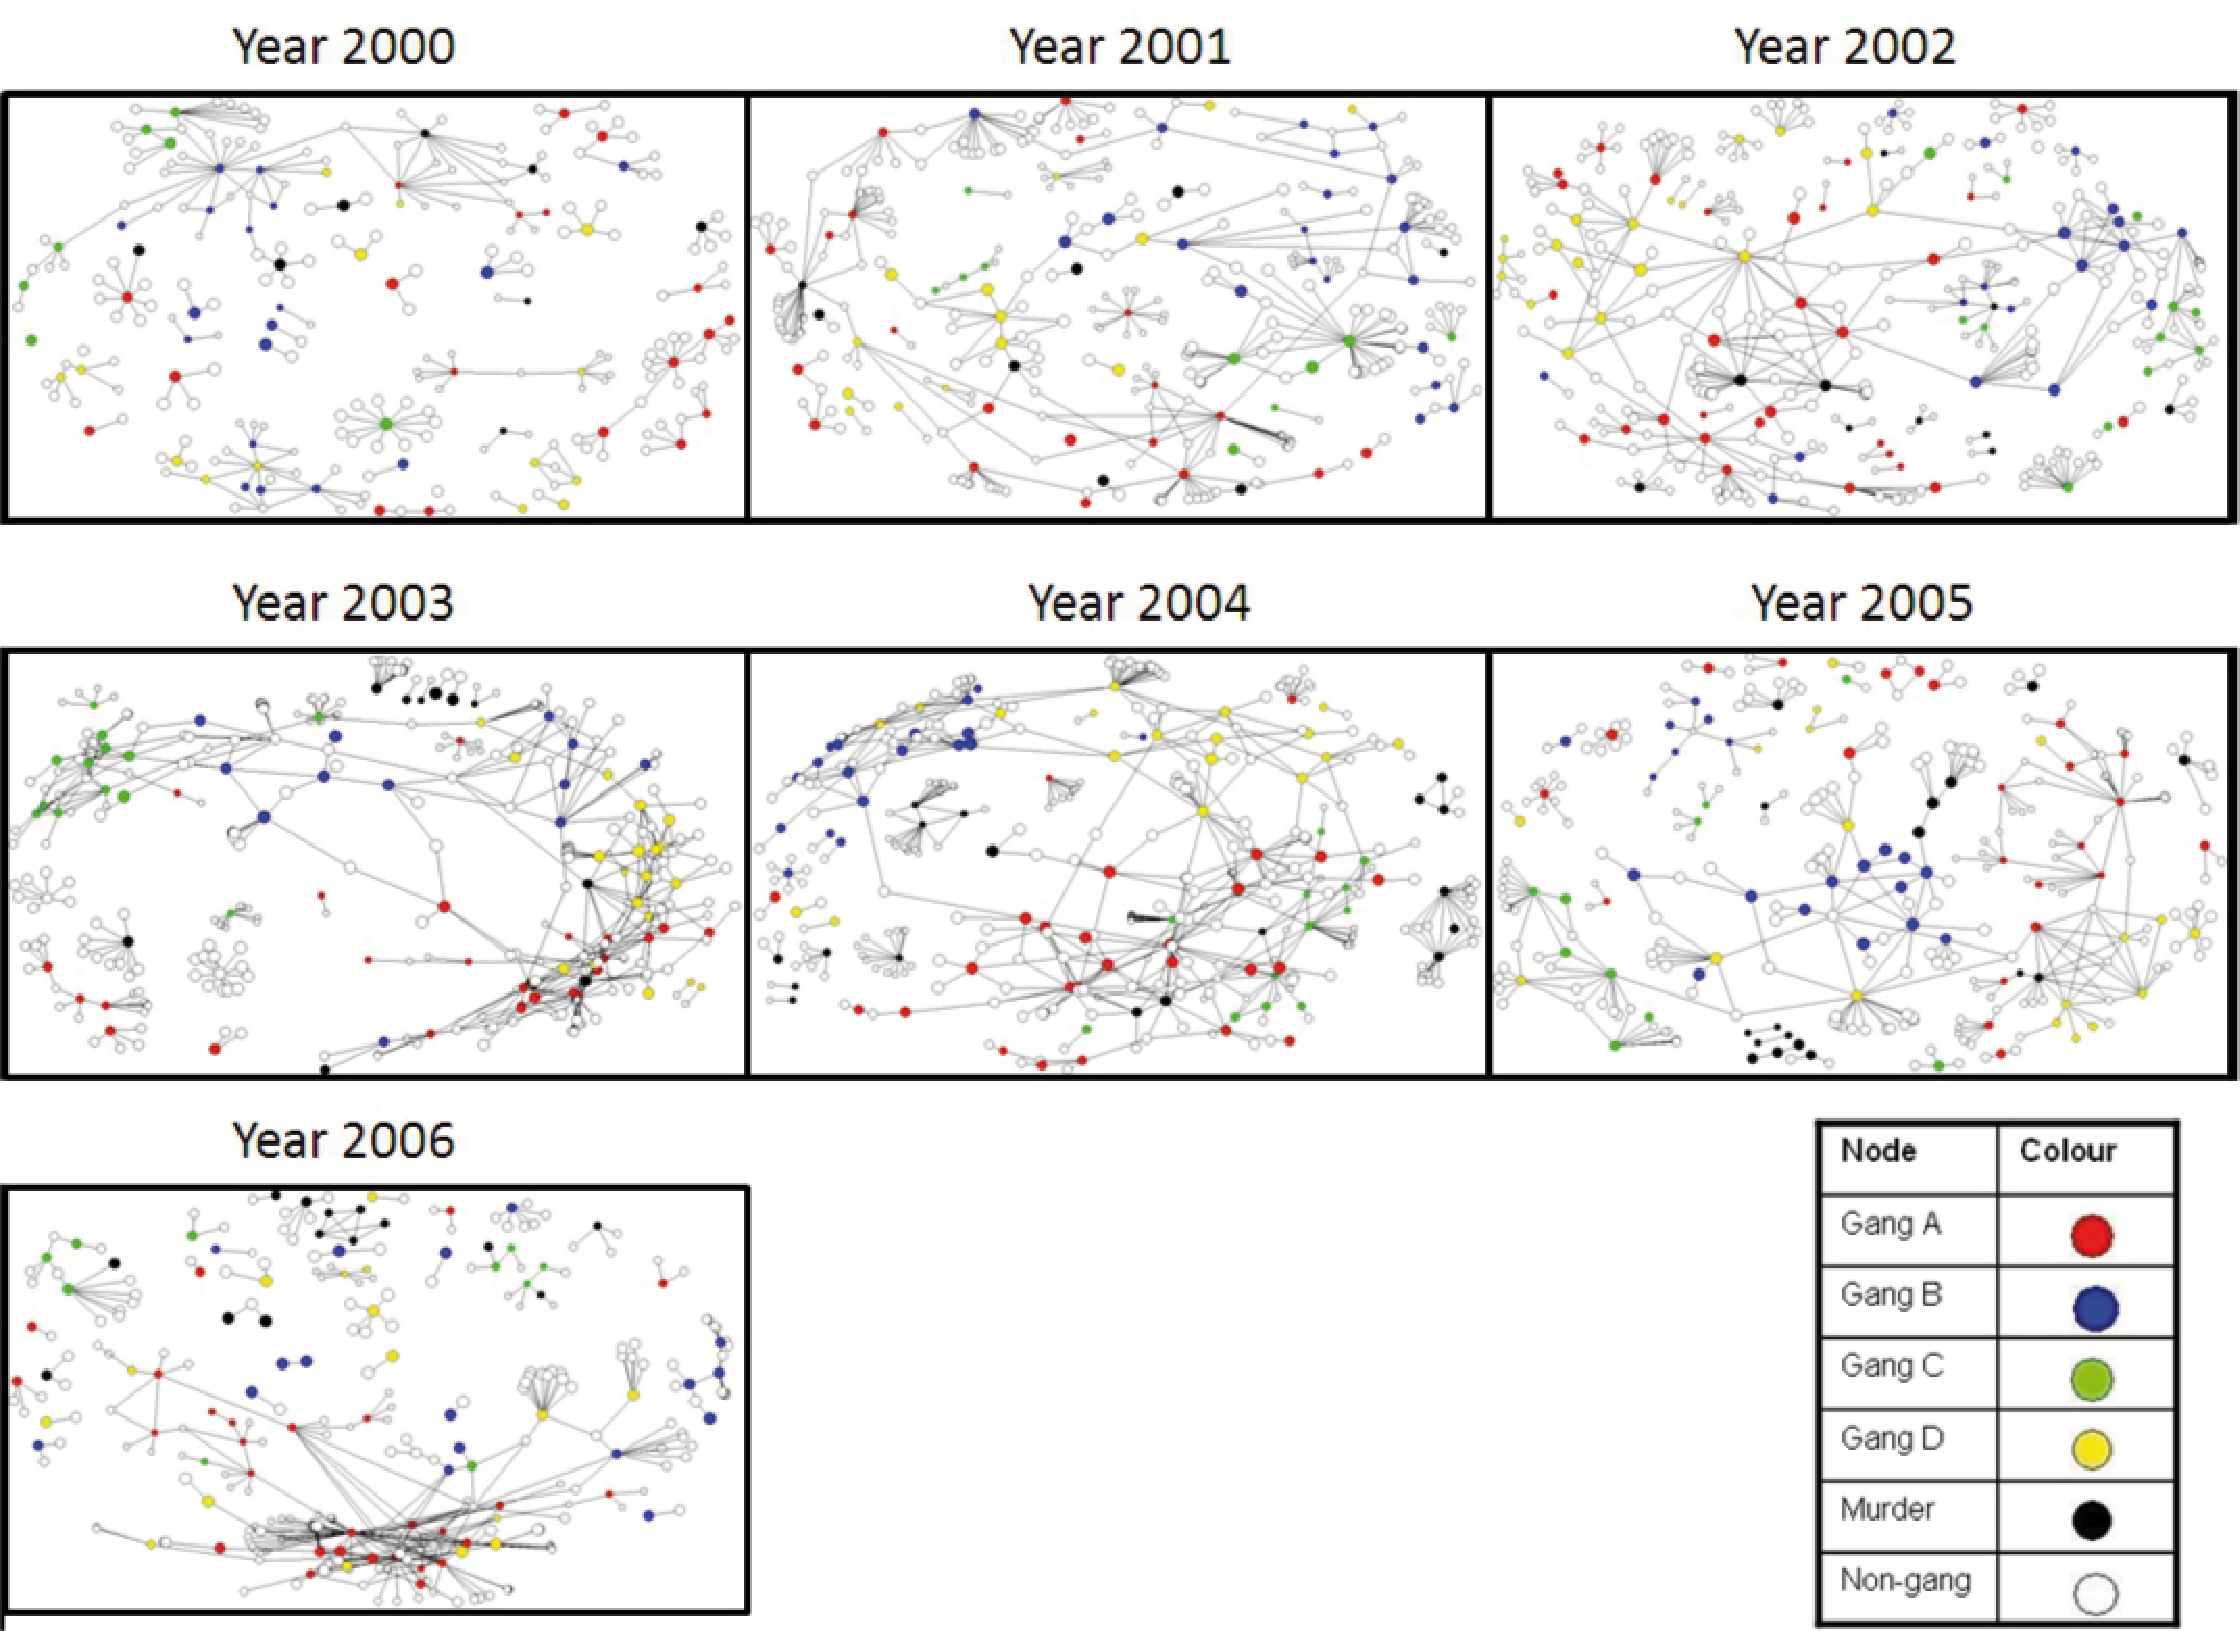
\includegraphics[width=0.9\paperwidth]{../images/all.pdf}
            };
        \end{tikzpicture}
     \end{frame}
}

\begin{frame}
\frametitle{Specific Gang Roles}
\begin{itemize}
\item {\textbf{Leader:}}
\begin{itemize}
\item responsible for recruiting new members
\end{itemize}
\item {\textbf{Provider:}}
\begin{itemize}
\item an individual either internal or external to the gang able to
  supply firearms and/or ammunition
\end{itemize}
\item {\textbf{Enforcers/Riders:}}
\begin{itemize}
\item nominated individuals who are active gunmen for the gang
\end{itemize}
\item {\textbf{Runners/Dealers:}}
\begin{itemize}
\item members of the gang who distribute/supply drugs, usually on the
  leader's behalf; younger members of the group
\end{itemize}
\end{itemize}
\end{frame}

\begin{frame}
\frametitle{Link Analysis}
\begin{center}
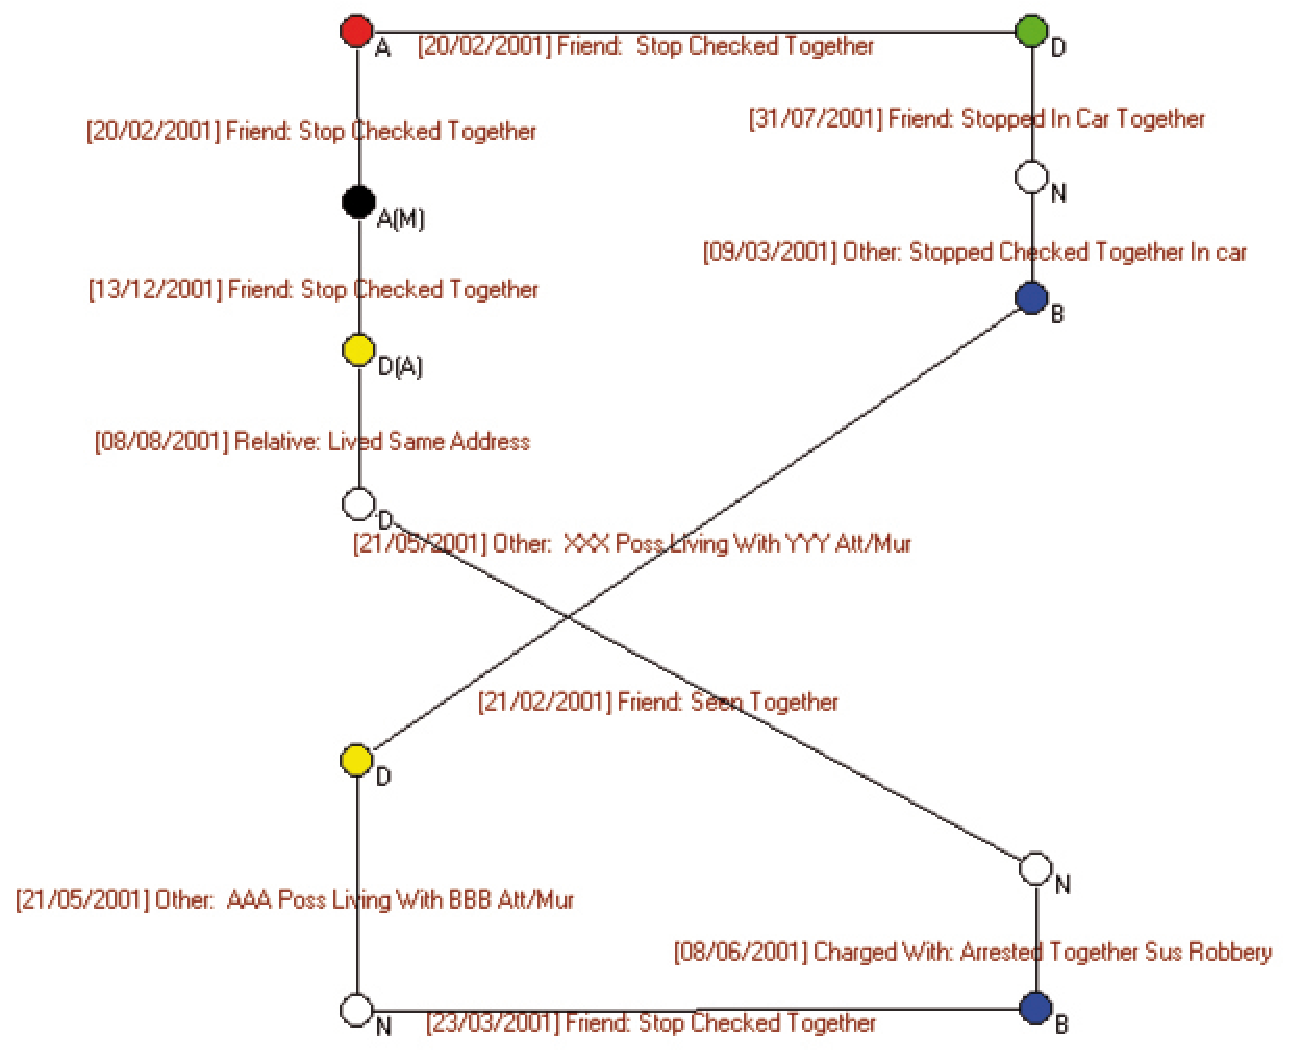
\includegraphics[width=0.48\textwidth]{../images/chain2001.pdf}
\hfill
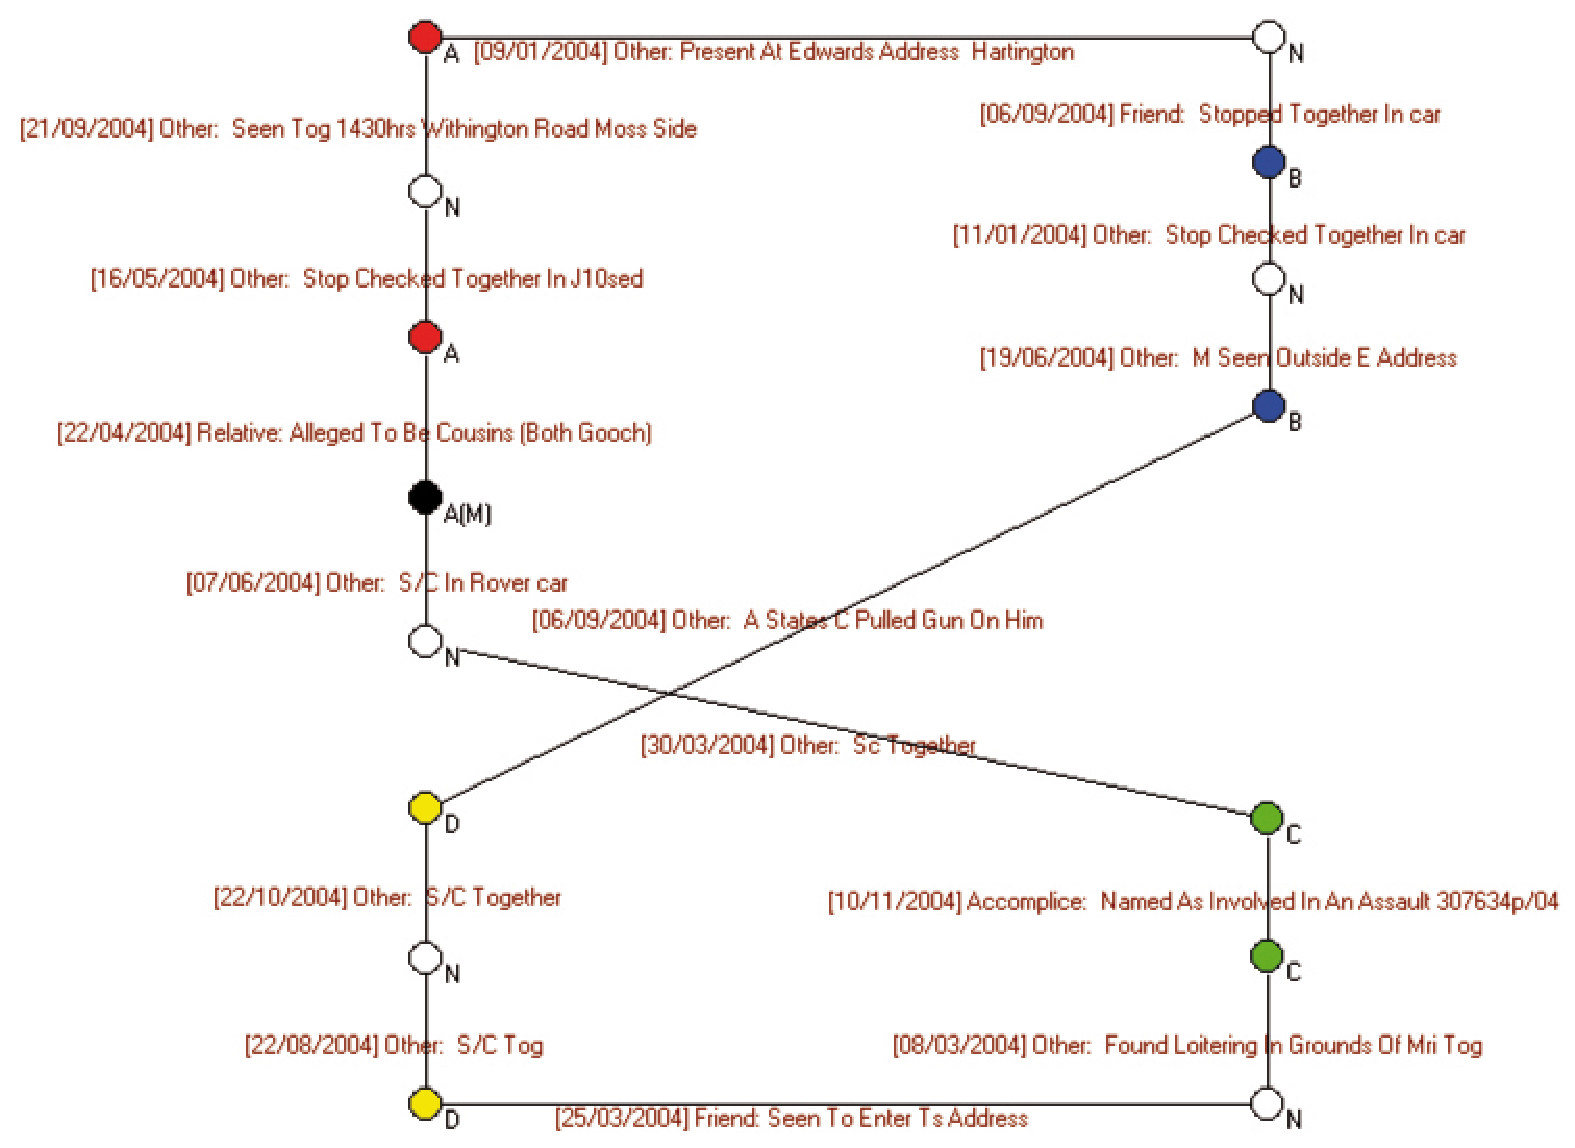
\includegraphics[width=0.48\textwidth]{../images/chain2004.pdf}
\end{center}
\scriptsize{{\textbf{Cycle (2001).}} The tension is between Gangs A
(red), B (blue), C (green) and D (yellow). A(M) is a member of the
Gooch gang (Gang A), however they are coloured black to represent the
crime of murder.}
\end{frame}

{ % all template changes are local to this group.
    \setbeamertemplate{navigation symbols}{}
    \begin{frame}[plain]
        \begin{tikzpicture}[remember picture,overlay]
            \node[at=(current page.center)] {
                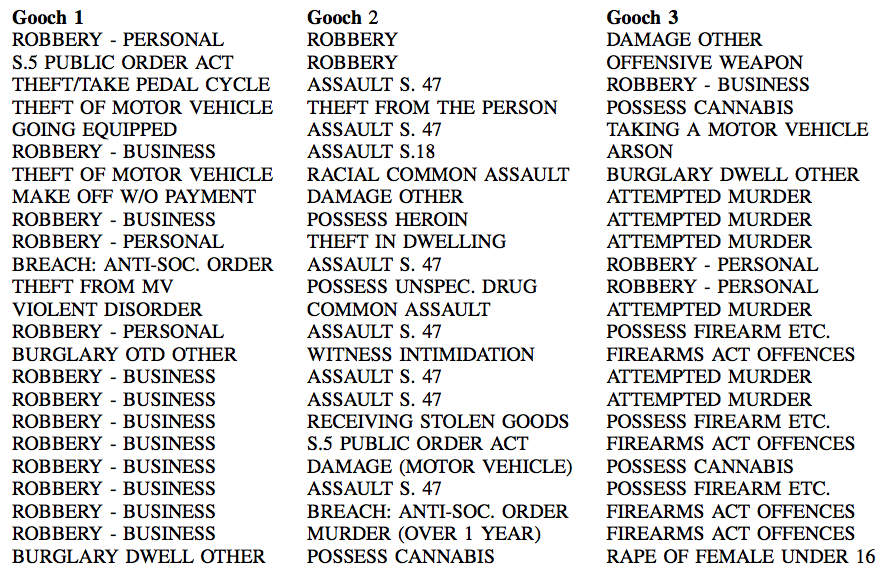
\includegraphics[width=0.9\paperwidth]{../images/offenderhistories.png}
            };
        \end{tikzpicture}
     \end{frame}
}

\begin{frame}
\frametitle{Gun Gangs}
\begin{itemize}
\item The picture painted by the initial social network plot is
somewhat misleading...
\item In the gun gangs, the police-held hypothesis of two rival sets
  of gangs is potentially a misrepresentation of the much more complex
  sets of smaller cliques and fluid changes within the larger gang
  structures.
\item {\textbf{Extremely rich dataset}}; more processing and analysis to follow
\end{itemize}
\end{frame}

\subsection{Retail Theft}

\begin{frame}
\frametitle{Retail Theft}
\begin{itemize}
\item Unique database from the {\textbf{UK's North East Retail Crime Partnership (NERCP)}}
\item Partnership between:
\begin{itemize}
\item 29 retail chains
\item 11 shopping centres
\item 6 town/city centre partnerships
\item 4 police forces in the NE of England (+ 11 further forces)
\end{itemize}
\item Information on over 30,000 offenders and 102,000 incidents in
  any 12 month period
\item Complex data of retail crime, with a fraction of known
  gangs, presents its own particular challenges -- how to make use of
  detailed intelligence on individuals (in textual format) and
  combine with mining of the social networks.
\end{itemize}
\end{frame}

% { % all template changes are local to this group.
%     \setbeamertemplate{navigation symbols}{}
%     \begin{frame}[plain]
%         \begin{tikzpicture}[remember picture,overlay]
%             \node[at=(current page.center)] {
%                 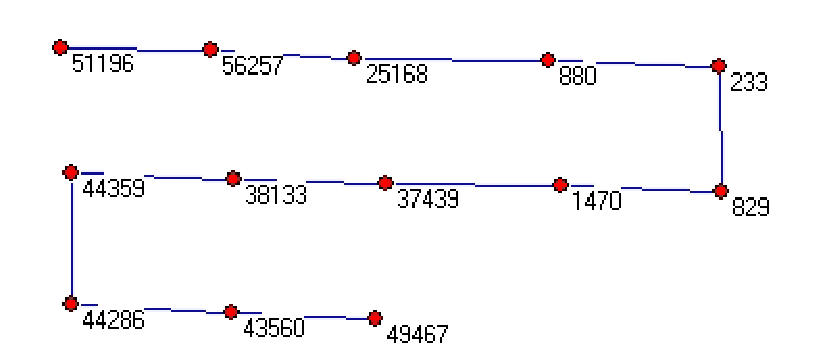
\includegraphics[width=0.9\paperwidth]{../images/path1.pdf}
%             };
%         \end{tikzpicture}
%      \end{frame}
% }

% { % all template changes are local to this group.
%     \setbeamertemplate{navigation symbols}{}
%     \begin{frame}[plain]
%         \begin{tikzpicture}[remember picture,overlay]
%             \node[at=(current page.center)] {
%                 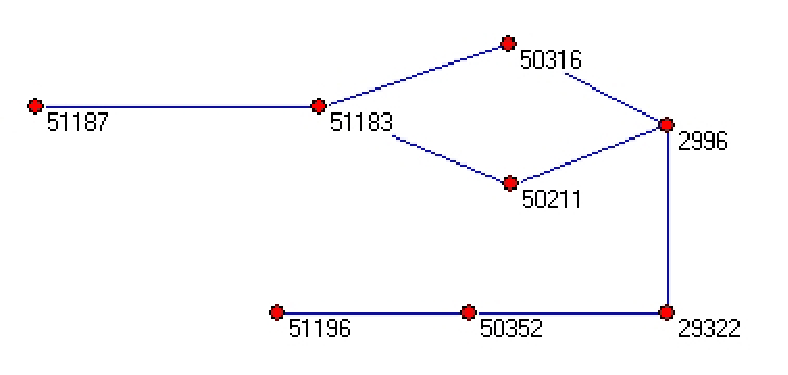
\includegraphics[width=0.9\paperwidth]{../images/path2.pdf}
%             };
%         \end{tikzpicture}
%      \end{frame}
% }

% { % all template changes are local to this group.
%     \setbeamertemplate{navigation symbols}{}
%     \begin{frame}[plain]
%         \begin{tikzpicture}[remember picture,overlay]
%             \node[at=(current page.center)] {
%                 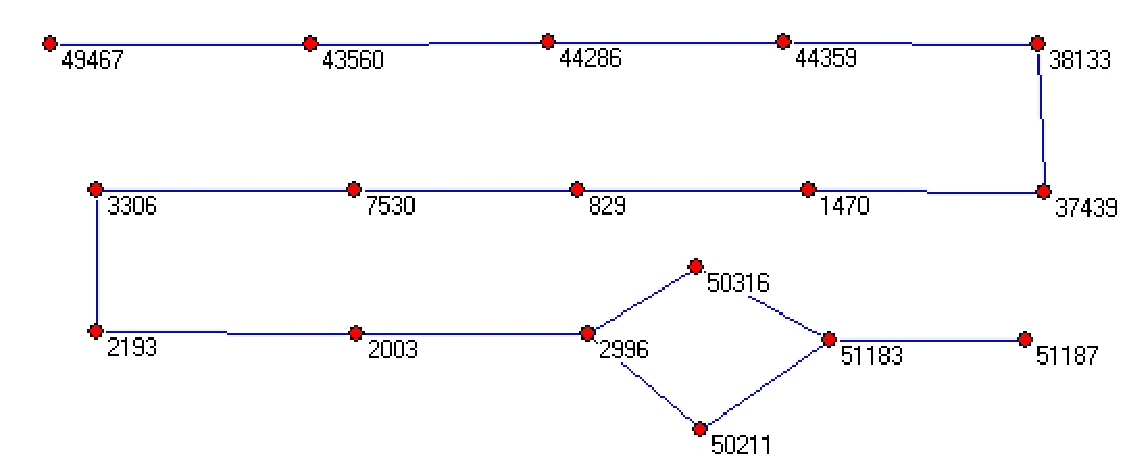
\includegraphics[width=0.9\paperwidth]{../images/path3.pdf}
%             };
%         \end{tikzpicture}
%      \end{frame}
% }

\begin{frame}
\begin{center}
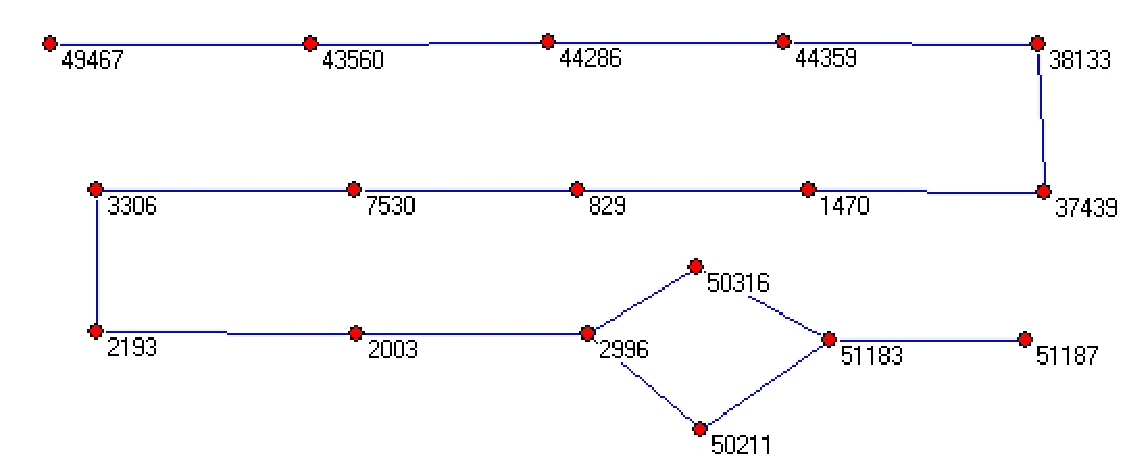
\includegraphics[width=0.9\paperwidth]{../images/path3.pdf}
\end{center}
\scriptsize{{\textbf{Shortest path between Offender 51196 (Gang SEA)
      and Offender 49467 (Gang CM).}}}
\end{frame}


\section{Conclusions and Future Work}

\begin{frame}
\frametitle{Conclusions and Future Work}
\begin{itemize}
\item The picture painted by the initial social network plot is somewhat
  misleading in all three cases we have presented:
\begin{itemize}
\item {\textbf{Burglary:}} requires spatial data
\item {\textbf{Gun Gangs:}} pre-existing police understanding of the gangs, not
  complex enough
\item {\textbf{Retail Theft:}} complex, fraction of known gangs, individual intelligence
\end{itemize}
\pause
\item How to represent the changing nature of an individual is
  something we have looked at elsewhere, and will continue to do so
\pause
\item Potential for shaping and influence policy in this area in
  the UK
\pause
\item Also see: {\emph{Measuring UK Crime Gangs}} (ASONAM 2014, S9)
\end{itemize}
\end{frame}

\begin{frame}
\frametitle{Acknowledgements}
\begin{itemize}
\item Acknowledge contributions from:
\begin{itemize}
\item West Midlands Police, UK
\item Greater Manchester Police, UK
\item North East Retail Crime Partnership (NERCP)\newline
\end{itemize}
\item Papers and presentations:
  \url{https://github.com/tomcrick/FOSINT-SI2014}\\
\url{https://github.com/tomcrick/ASONAM2014}\newline
\item Contact: \url{http://drtomcrick.com}

\end{itemize}
\end{frame}


\end{document}
